\documentclass[11pt,a4paper]{article}
\usepackage[utf8]{inputenc}
\usepackage[T1]{fontenc}
\usepackage[english]{babel}
\usepackage[english]{isodate}
\usepackage[paper=a4paper]{geometry}
\newgeometry{top=3.5cm,bottom=2.5cm,right=2.5cm,left=2.5cm}
\usepackage{graphicx}
\usepackage{comment}
\usepackage{fancyhdr}
\usepackage{framed}
\usepackage{lastpage}
\usepackage[hidelinks]{hyperref}
\usepackage{tabularx}
\usepackage[table]{xcolor}
\usepackage{enumitem}
\usepackage{mdwlist}
\usepackage{placeins}
\usepackage{amsmath}
\usepackage{amsfonts}
\usepackage{xcolor}
\usepackage{listings}

\usepackage{booktabs}
\usepackage{caption}
\usepackage{longtable}
\captionsetup[table]{skip=10pt} % Aggiunge spazio tra la didascalia della tabella e il contenuto della tabella
\usepackage{array} % Per personalizzare le righe della tabella


\begin{document}


\newcommand{\imageLabel}[4]{ % 1 image 2 caption 3 size
	\begin{figure}[h!]
		\centering
		\includegraphics[width=#3\textwidth]{#1} 
		\caption{#2}
		\label{fig:#4}
	\end{figure}
	\FloatBarrier
}
\renewcommand{\figurename}{Figura}
\renewcommand{\tablename}{Tabella}

\newcommand{\titolo}  {Laboratorio di Algoritmi

e Strutture Dati}
\newcommand{\sottotitolo} {Confronto metodi per calcolare LCS tra due stringhe}
\newcommand{\nome}    {Federico Donati}





\newcommand{\image}[3]{ % 1 image 2 caption 3 size
	\begin{figure}[h!]
		\centering
		\includegraphics[width=#3\textwidth]{#1} 
		\caption{#2}
	\end{figure}
	\FloatBarrier
}

\newcommand{\imageLabel}[4]{ % 1 image 2 caption 3 size
	\begin{figure}[h!]
		\centering
		\includegraphics[width=#3\textwidth]{#1} 
		\caption{#2}
		\label{fig:#4}
	\end{figure}
	\FloatBarrier
}
\newcommand{\Z}{\mathbb{Z}}

\pagenumbering{Alph}
\begin{titlepage}
	\begin{center}
		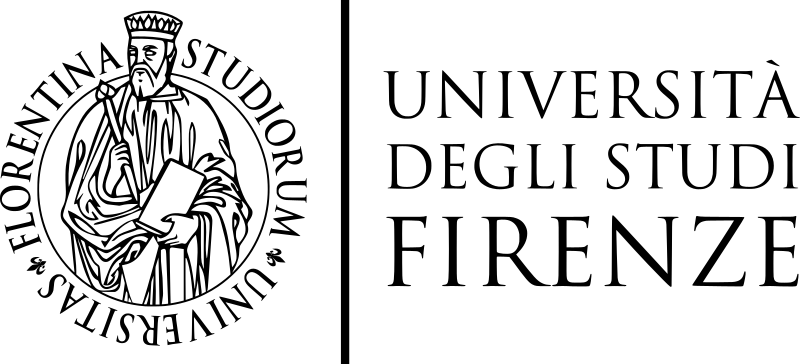
\includegraphics[width=0.5\textwidth]{Logo_universita_firenze.svg.png}
		
		\vspace*{1cm}
		\LARGE
		\textit{Università degli Studi di Firenze \\ \center Anno: 2024}
		
		\vspace{0.5cm}
		\Huge{\titolo}
  
        \vspace{0.5 cm}
		\textbf{\sottotitolo}\\
  
        
		
		\line(1,0){280}
		
		\vspace{0.5 cm}
		\LARGE {\nome}
		
		\vfill
		
	\end{center}
	
	
\end{titlepage}


\renewcommand{\headheight}{14pt}

\pagestyle{fancy}
\lhead{}
\chead{}
\rhead{\textbf{\sottotitolo}}
\cfoot{}
\renewcommand{\headrulewidth}{0.4pt}
\renewcommand{\footrulewidth}{0.4pt}

\renewcommand{\labelitemi}{$\diamond$}
\renewcommand{\labelitemii}{$\bullet$}
\renewcommand{\labelitemiii}{$\circ$}

\setlist{itemsep=0pt}

\setlength{\parindent}{0cm}



\pagenumbering{gobble}
\renewcommand{\contentsname}{Index}
\tableofcontents %%questo è l'indice vero e proprio%%
\newpage
\pagenumbering{arabic}



\rfoot{\thepage\ di \pageref{LastPage}}



\definecolor{mygreen}{rgb}{0,0.6,0}
\definecolor{mygray}{rgb}{0.5,0.5,0.5}
\definecolor{mymauve}{rgb}{0.58,0,0.82}

\lstset{ %
	backgroundcolor=\color{white},   
	basicstyle=\footnotesize,        
	breakatwhitespace=false,        
	breaklines=true,                 
	captionpos=b,                    
	commentstyle=\color{mygreen},    
	deletekeywords={...},           
	escapeinside={\%*}{*)},          
	extendedchars=true,              
	frame=single,	                   
	keepspaces=true,                 
	keywordstyle=\color{blue},       
	language=Octave,                
	morekeywords={*,...},           
	numbers=left,                  
	numbersep=5pt,                   
	numberstyle=\tiny\color{mygray}, 
	rulecolor=\color{black},         
	showspaces=false,                
	showstringspaces=false,          
	showtabs=false,                  
	stepnumber=2,                    
	stringstyle=\color{mymauve},    
	tabsize=2,	                  
	title=\lstname                   
}


\section {Introduzione}
In questa relazione analizzeremo vari metodi per calcolare LCS ("Longest Common Subsequence"), ovvero la sottosequenza più lunga comune a due sequenze.Ciò significa andare a risolvere il seguente problema:

Date 2 sequenze, $X =< x_{1}, . . . , x_{m} > e Y =< y_{1}, . . . , y_{n} >$
trovare una sottosequenza comune ad X e Y di lunghezza massima.

Una sottosequenza di una sequenza è definita comme una sequenza privata di 0 o più dei suoi elementi.

Per farlo,utilizzeremo l'algoritmo "forza-bruta",l'algoritmo ricorsivo, l'algoritmo ricorsivo con memoization e infine l'algoritmo iterativo (bottom up).

Di ciascun metodo verrà fornita una spiegazione dell'algoritmo e del suo funzionamento, l'implementazione dell'algoritmo, e verranno eseguiti e descritti alcuni test che metteranno in evidenza le varie caratteristiche. 

\section {Algoritmo "forza-bruta"}
\label{bruteforce cap}
Date due sequenze X e Y , l'algoritmo "forza-bruta" consiste nel controllare per ciascuna sottosequenza di X se essa è anche sottosequenza di Y, e ovviamente scegliere la più lunga.

Le sottosequenze di X da controllare sono quindi $2^m$ , con "m" lunghezza di X.

La complessità per controllare ogni sottosequenza è $\Theta(n)$, con "n" lunghezza di Y, che corrisponde a dover scorrere tutta la sequenza Y per ogni sottoseuenza di X.

Si arriva dunque ad una complessità di \Theta($n * 2^m$).

L'algoritmo "brute-force" può essere implementato in Python come segue:

\lstset{language=Python} % Imposta il linguaggio per il blocco di codice

\begin{lstlisting}
def Lcs_bruteforce(X,Y):
    if len(X)==0:
        return 0
    maxi=0
    for i in range(0,len(X)):
        s=X[0:i]+X[i+1:len(X)]
        maxi=max(maxi,Lcs_bruteforce(s,Y))
    if X in Y:
            maxi=len(X)
    return maxi     
\end{lstlisting}
Eseguiamo un test su due stringhe contenenti entrambe 12 caratteri casuali, e notiamo che già con una lunghezza così modesta il tempo impiegato è notevole (oltre 10 minuti su un computer portatile con processore Intel Core i5) e questo ci fa capire quanto inefficiente sia questo metodo, la cui complessità come descritto precedentemente contiene un termine che cresce esponenzialmente al crescere della lughezza della prima stringa.

\begin{table}[htbp]
    \centering
    \caption{Lcs brute-force test}
    \begin{tabular}{|c|c|}
        \hline
        Dim X e Y & tempo impiegato (s) \\
        \hline
        1 & 0.00 \\
        2 & 0.00 \\
        3 & 0.00 \\
        4 & 0.00 \\
        5 & 0.00 \\
        6 & 0.00 \\
        7 & 0.01\\
        8 & 0.05 \\
        9 & 0.36 \\
        10 & 4.16 \\
        11 & 45.96\\
        12 & 621.33 \\
        
        \hline
    \end{tabular}
\end{table}

Il seguente grafico (Figura \ref{fig:lcs_bruteforce_test})ci mostra il crescere del tempo impiegato al crescere della dimensione delle stringhe:

\begin{figure}[htbp]
    \centering
    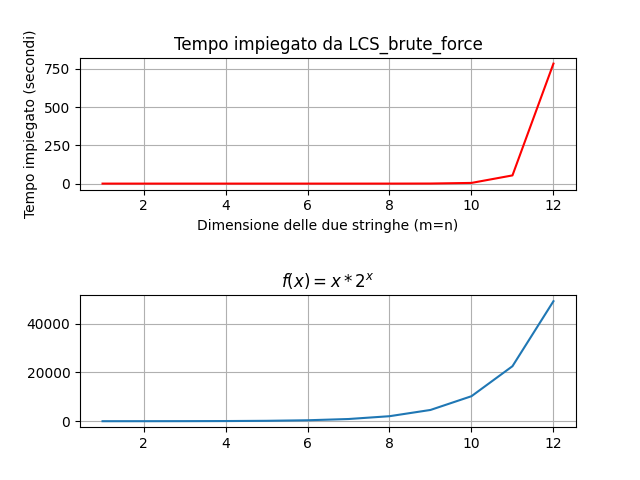
\includegraphics[width=0.5\textwidth]{lcs bruteforce test.png}
    \caption{Test algoritmo brute-force}
    \label{fig:lcs_bruteforce_test}
\end{figure}

Come si può notare la crescita della funzione è molto ripida (dovuta alla complessità) e ciò testimonia l'inefficienza di questo algoritmo.

\section{Algoritmo ricorsivo}
\subsection{Lcs-recursive}
\label{Lcs-recursive cap}
Un altro metodo che possiamo utilizzare per calcolare Lcs tra due stringhe è utilizzare un algoritmo ricorsivo, che si basa sul principio di programmazione dinamica "divide-et-impera".

Per arrivare a formulare questa soluzione dobbiamo innanzitutto definire una sottostruttura ottima; date due stringhe X e Y, denotiamo con $ X_{i}$ il prefisso di X con i elementi: 

$< x_{1}, . . . , x_{i} >$, e con $Y_{j}$ il prefisso di Y con j elementi: $< y_{1}, . . . , y_{j} >$.

A questo punto possiamo applicare il teorema secondo il quale date le sequenze

X =$< x_{1}, . . . , x_{m} >$ e 
Y =$< y_{1}, . . . , y_{n} >$
sia Z =$< z_{1}, . . . , z_{k} >$ una qualsiasi LCS di X e Y:

\begin{itemize}
	\item Se $x_{m} = y_{n}$, allora $z_{k} = x_{m} = y_{n}$ e $Z_{k{-}1}}$ è una LCS di $X_{m{-}1}$ e $Y_{n{-}1}$
	\item $x_{m} \neq y_{n}$, allora $z_{k} \neq x_{m}$ implica che Z è una LCS di $X_{m{-}1}$ e Y
	\item Se $x_{m} \neq yn$, allora $z_{k} \neq y_{n}$ implica che Z è una LCS di X e Y_{n{-}1}$
\end{itemize}

Nel caso in cui $x_{m} = y_{n}$ dovremo quindi esaminare un sottoproblema, altrimenti dovremo esaminarne due per giungere alla soluzione.

Questo porta ad una complessità pari a $\Theta(2^n)$, dove n è la lunghezza di X (=m lunghezza di Y).

Risulta quindi che questo algoritmo è molto più efficiente rispetto a quello brute-force visto precedentemente (capitolo \ref{bruteforce cap})


Non ci resta infine che calcolare la soluzione in modo ricorsivo:
\[
\left.
\begin{aligned}
c[i, j] &= \begin{cases}
0 & \text{se } i = 0 \text{ o } j = 0 \text{ (X o Y è vuota)} \\
c[i-1, j-1] + 1 & \text{se } i, j > 0 \text{ e } x_i = y_j \\
\max(c[i, j-1], c[i-1, j]) & \text{se } i, j > 0 \text{ e } x_i \neq y_j
\end{cases}
\end{aligned}
\right.
\]

Calcoliamo la lunghezza della soluzione ottima con la seguente implementazione in Python dell'algoritmo ricorsivo:
\begin{lstlisting}
   def Lcs_recursive(X,Y):
    m=len(X)
    n=len(Y)
    if m==0 or n==0:
        return 0
    if X[m-1]==Y[n-1]:
        return 1 + Lcs_recursive(X[:-1],Y[:-1])
    else: 
        return max(Lcs_recursive(X,Y[:-1]),Lcs_recursive(X[:-1],Y))
    
\end{lstlisting}
Verifichiamo l'andamento esponenziale $\Theta(2^n)$ dell' algoritmo ricorsivo per determinare Lcs tra due stringhe al crescere della dimensione delle due stringhe.

La dimensione delle due stringhe è la medesima, e cresce di 1 unità alla volta fino a 15.
\newpage
\begin{longtable}{|c|c|c|}
    \caption{Dati con terza colonna troncata a due cifre decimali}\\
    \hline
    Dimensione stringhe & Dimensione Lcs & Tempo impiegato (s) \\
    \hline
    \endfirsthead
    \multicolumn{3}{c}%
    {\tablename\ \thetable\ -- \textit{continua dalla pagina precedente}} \\
    \hline
    Dimensione stringhe & Dimensione Lcs & Tempo impiegato (s) \\
    \hline
    \endhead
    \hline \multicolumn{3}{r}{\textit{Continua nella pagina successiva}} \\
    \endfoot
    \hline
    \endlastfoot
    1 & 0 & 0.00 \\
    2 & 0 & 0.00 \\
    3 & 0 & 0.00 \\
    4 & 0 & 0.00 \\
    5 & 0 & 0.00 \\
    6 & 0 & 0.00 \\
    7 & 1 & 0.00 \\
    8 & 0 & 0.00 \\
    9 & 0 & 0.03 \\
    10 & 1 & 0.07 \\
    11 & 1 & 0.23 \\
    12 & 2 & 0.60 \\
    13 & 2 & 2.85 \\
    14 & 1 & 12.62 \\
    15 & 2 & 45.35 \\
\end{longtable}
\begin{figure}[htbp]
    \centering
    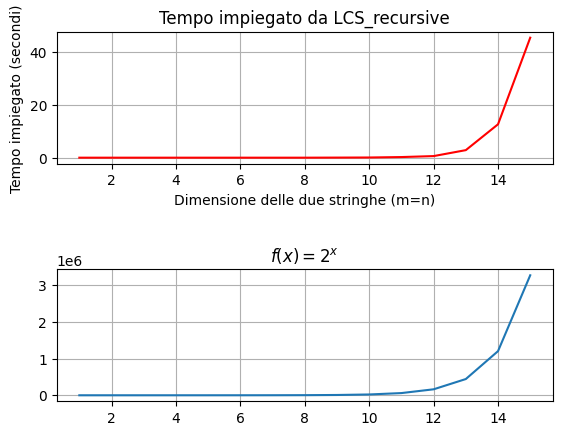
\includegraphics[width=0.5\textwidth]{LCS_recursive test.png}
    \caption{Test algoritmo ricorsivo}
    \label{fig:lcs_recursive_test}
\end{figure}

Come mostrato dal grafico (Figura \ref{fig:lcs_recursive_test}) questo algoritmo ha una complessità esponenziale $\Theta(2^n)$ , con n(=m) lunghezza delle due stringhe X e  Y.

L'algoritmo ricorsivo appena descritto tuttavia può generare chiamate ricorsive con stesso input che vengono ripetute andando a peggiorare l'efficienza della funzione, come mostrato dall'albero di ricorsione(figura \ref{fig:lcs_recursion_tree}).

\begin{figure}[htbp]
    \centering
    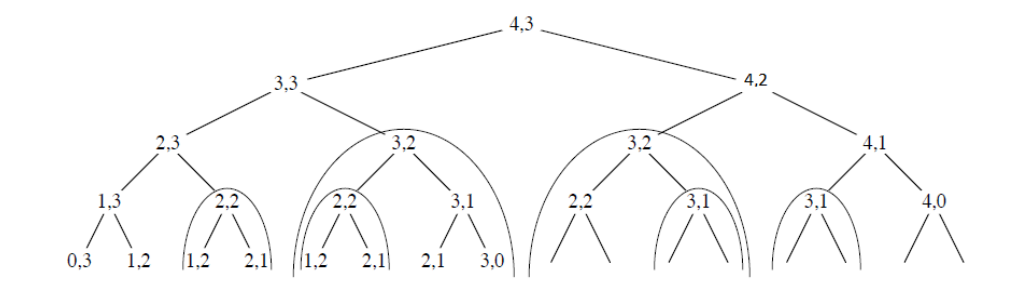
\includegraphics[width=\textwidth]{Lcs recursion tree.png}
    \caption{Albero di ricorsione algoritmo LCS-recursive}
    \label{fig:lcs_recursion_tree}
\end{figure}

Per questo possiamo realizzare un algoritmo che memorizza i risultati ottenuti per ogni input in una tabella per evitare di chiamare più volte la funzione ricorsiva con il medesimo input.
\subsection{Lcs-recursive-memoization}
L'alternativa proposta permette di ridurre il tempo di esecuzione dell'algoritmo evitando di ripetere chiamate ricorsive con stesso imput. vediamo un esempio di codice python che permette di implementare questo algoritmo con memoria:
\newpage
\begin{lstlisting}
   def Lcs_recursive_memoization(X,Y):
    m=len(X)
    n=len(Y)
    lengths = [[-1] * (n+1 ) for _ in range(m+1)]
    return Lcs_rec_mem_aux(X,Y,m,n,lengths)

def Lcs_rec_mem_aux(X,Y,x,y,lens):
    if x==0 or y==0:
        return 0
    if lens[x][y] >= 0 :
        return lens[x][y] 
    q=-1
    if X[x-1]==Y[y-1]:
        q= 1 + Lcs_rec_mem_aux(X,Y,x-1,y-1,lens)
    else: 
        q= max(q,Lcs_rec_mem_aux(X,Y,x-1,y,lens),Lcs_rec_mem_aux(X,Y,x,y-1,lens))
    lens[x][y]=q
    return q
\end{lstlisting}

La complessità di questo algoritmo è $\Theta(n*m)$,(con n dimensione di X e m dimensione di Y) , ovvero quadratica ($\Theta(n^2)$) nel caso di stringhe di stessa dimensione. Possiamo notare quindi che questa modifica ha influito notevolmente sull'efficienza della funzione, come dimostra il seguente test eseguito su stringhe con dimensione uguale crescente a intervalli di 100 da 1 a 5000. 

\begin{longtable}{|c|c|c|}
    \caption{Dati con terza colonna troncata a due cifre decimali}\\
    \hline
    Dimensione stringhe & Dimensione Lcs & Tempo impiegato (s) \\
    \hline
    \endfirsthead
    \multicolumn{3}{c}%
    {\tablename\ \thetable\ -- \textit{continua dalla pagina precedente}} \\
    \hline
    Dimensione stringhe & Dimensione Lcs & Tempo impiegato (s) \\
    \hline
    \endhead
    \hline \multicolumn{3}{r}{\textit{Continua nella pagina successiva}} \\
    \endfoot
    \hline
    \endlastfoot
    1 & 0 & 0.0 \\
    201 & 39 & 0.04 \\
    401 & 84 & 0.10 \\
    601 & 128 & 0.22 \\
    801 & 175 & 0.38 \\
    1001 & 219 & 0.58 \\
    1201 & 264 & 0.89 \\
    1401 & 309 & 1.21 \\
    1601 & 350 & 1.70 \\
    1801 & 393 & 2.00 \\
    2001 & 454 & 2.52 \\
    2201 & 484 & 3.44 \\
    2401 & 525 & 5.28 \\
    2601 & 565 & 6.56 \\
    2801 & 626 & 6.75 \\
    3001 & 669 & 7.36 \\
    3201 & 721 & 9.10 \\
    3401 & 765 & 12.63 \\
    3601 & 800 & 13.20 \\
    3801 & 840 & 10.93 \\
    4001 & 889 & 11.15 \\
    4201 & 930 & 12.25 \\
    4401 & 978 & 13.50 \\
    4601 & 1005 & 15.42 \\
    4801 & 1075 & 16.28 \\
    5001 & 1104 & 17.70 \\
\end{longtable}


\begin{figure}[htbp]
    \centering
    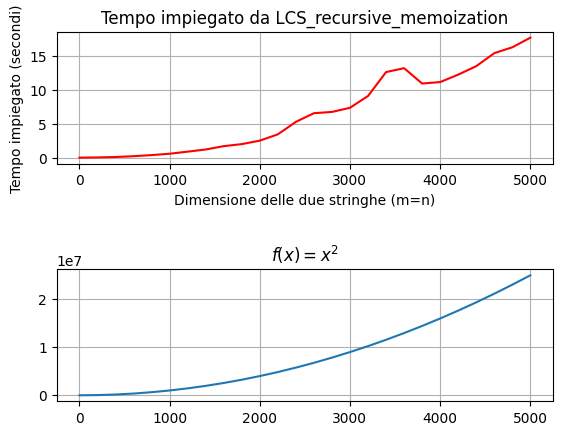
\includegraphics[width=0.5\textwidth]{LCS_recursive_mem test.png}
    \caption{Test algoritmo ricorsivo con memoization}
    \label{fig:lcs_recursive_mem_test}
\end{figure}
\newpage
Il grafico (figura\ref{fig:lcs_recursive_mem_test}) mostra l'andamento quadratico dell'algoritmo.

\section{Algoritmo iterativo}
Nei capitoli precedenti abbbiamo analizzato algoritmi più o meno efficienti per il calcolo della lunghezza dell'LCS tra due stringhe di uguale dimensione X e Y. Vediamo ora un algoritmo iterativo che ci consente di stabilire la lunghezza dell'LCS e allo stesso tempo da quali caratteri è formata. L'algoritmo consiste nel rappresentare due tabelle c e b, dove rispettivamente verranno inseriti la lunghezza dell'LCS e il percorso eseguito per determinarla. La complessità di questo algoritmo è $\Theta(n^2)$.

Il codice dell'algoritmo è il seguente:

\begin{lstlisting}
    def LCS_Length(X, Y):
    m = len(X)
    n = len(Y)
    b = [["" for _ in range(n)] for _ in range(m)]
    c = [[0 for _ in range(n+1)] for _ in range(m+1)]
    
    for i in range(1, m+1):
        c[i][0] = 0
    for j in range(n+1):
        c[0][j] = 0
        
    for i in range(1, m+1):
        for j in range(1, n+1):
            if X[i-1] == Y[j-1]:
                c[i][j] = c[i-1][j-1] + 1
                b[i-1][j-1] = "↖"
            elif c[i-1][j] >= c[i][j-1]:
                c[i][j] = c[i-1][j]
                b[i-1][j-1] = "↑"
            else:
                c[i][j] = c[i][j-1]
                b[i-1][j-1] = "←"
                
    return c, b
\end{lstlisting}


c[i, j] (Tabella \ref{output matrice c}) contiene la lunghezza ottima di LCS per $ X_{i}$ e $Y_{j}$.

b[i, j] (Tabella \ref{output matrice b}) indica la strada seguita (il sottoproblema) per risolvere
LCS di $X_{i}$ e $Y_{j}$.

Se b[i, j] = $\nwarrow$ , ho esteso LCS di un carattere ($x_{i} = y_{j}$).

LCS contiene $x_{i}$ (e $y_{j}$) in cui b[i, j] = $\nwarrow$.


Eseguiamo adesso un esempio con stringhe casuali di dimensione 12 per mostrare il funzionamento dell'algoritmo attraverso il seguente codice Python:
\begin{lstlisting}
n_values = list(range(1, 12))
time_values = []
X = ''.join(random.choices(string.ascii_letters + string.digits, k=12))
Y=''.join(random.choices(string.ascii_letters + string.digits, k=12))
start_time = time.time()
c, b = LCS_Length(X, Y)
print("Matrice c:")
for row in c:
    print(row)
print("\nMatrice b:")
for row in b:
    print(row)
#print(Lcs_bruteforce(X,Y))
end_time = time.time() 
elapsed_time = end_time - start_time
print(elapsed_time)
\end{lstlisting}

String X: "2GpBvhkb2YHA"


String Y: "VlYchJMG6tbW"

LCS: "hb"


\begin{table}[htbp]
    \centering
    \caption{output matrice c}
    \label{output matrice c}
    \begin{tabular}{|*{13}{c|}}
        \hline
        0 & 0 & 0 & 0 & 0 & 0 & 0 & 0 & 0 & 0 & 0 & 0 & 0 \\
        \hline
        0 & 0 & 0 & 0 & 0 & 0 & 0 & 0 & 0 & 0 & 0 & 0 & 0 \\
        \hline
        0 & 0 & 0 & 0 & 0 & 0 & 0 & 0 & 1 & 1 & 1 & 1 & 1 \\
        \hline
        0 & 0 & 0 & 0 & 0 & 0 & 0 & 0 & 1 & 1 & 1 & 1 & 1 \\
        \hline
        0 & 0 & 0 & 0 & 0 & 0 & 0 & 0 & 1 & 1 & 1 & 1 & 1 \\
        \hline
        0 & 0 & 0 & 0 & 0 & 0 & 0 & 0 & 1 & 1 & 1 & 1 & 1 \\
        \hline
        0 & 0 & 0 & 0 & 0 & 1 & 1 & 1 & 1 & 1 & 1 & 1 & 1 \\
        \hline
        0 & 0 & 0 & 0 & 0 & 1 & 1 & 1 & 1 & 1 & 1 & 1 & 1 \\
        \hline
        0 & 0 & 0 & 0 & 0 & 1 & 1 & 1 & 1 & 1 & 1 & 2 & 2 \\
        \hline
        0 & 0 & 0 & 0 & 0 & 1 & 1 & 1 & 1 & 1 & 1 & 2 & 2 \\
        \hline
        0 & 0 & 0 & 1 & 1 & 1 & 1 & 1 & 1 & 1 & 1 & 2 & 2 \\
        \hline
        0 & 0 & 0 & 1 & 1 & 1 & 1 & 1 & 1 & 1 & 1 & 2 & 2 \\
        \hline
        0 & 0 & 0 & 1 & 1 & 1 & 1 & 1 & 1 & 1 & 1 & 2 & 2 \\
        \hline
    \end{tabular}
\end{table}

\newpage
\begin{table}[htbp]
    \centering
    \caption{output matrice b}
    \label{output matrice b}
    \begin{tabular}{|*{12}{c|}}
        \hline
        ↑ & ↑ & ↑ & ↑ & ↑ & ↑ & ↑ & ↑ & ↑ & ↑ & ↑ & ↑ \\
        \hline
        ↑ & ↑ & ↑ & ↑ & ↑ & ↑ & ↑ & \nwarrow & ← & ← & ← & ← \\
        \hline
        ↑ & ↑ & ↑ & ↑ & ↑ & ↑ & ↑ & ↑ & ↑ & ↑ & ↑ & ↑ \\
        \hline
        ↑ & ↑ & ↑ & ↑ & ↑ & ↑ & ↑ & ↑ & ↑ & ↑ & ↑ & ↑ \\
        \hline
        ↑ & ↑ & ↑ & ↑ & ↑ & ↑ & ↑ & ↑ & ↑ & ↑ & ↑ & ↑ \\
        \hline
        ↑ & ↑ & ↑ & ↑ & \nwarrow & ← & ← & ↑ & ↑ & ↑ & ↑ & ↑ \\
        \hline
        ↑ & ↑ & ↑ & ↑ & ↑ & ↑ & ↑ & ↑ & ↑ & ↑ & ↑ & ↑ \\
        \hline
        ↑ & ↑ & ↑ & ↑ & ↑ & ↑ & ↑ & ↑ & ↑ & ↑ & \nwarrow & ← \\
        \hline
        ↑ & ↑ & ↑ & ↑ & ↑ & ↑ & ↑ & ↑ & ↑ & ↑ & ↑ & ↑ \\
        \hline
        ↑ & ↑ & \nwarrow & ← & ↑ & ↑ & ↑ & ↑ & ↑ & ↑ & ↑ & ↑ \\
        \hline
        ↑ & ↑ & ↑ & ↑ & ↑ & ↑ & ↑ & ↑ & ↑ & ↑ & ↑ & ↑ \\
        \hline
        ↑ & ↑ & ↑ & ↑ & ↑ & ↑ & ↑ & ↑ & ↑ & ↑ & ↑ & ↑ \\
        \hline
    \end{tabular}
\end{table}


Con un input di 12 elementi il tempo impiegato è stato di 0.00 secondi, decisamente migliore rispetto all'algoritmo "brute-force" (capitolo \ref{bruteforce cap}) o all'algoritmo ricorsivo (capitolo \ref{Lcs-recursive cap}

Vediamo adesso come si comporta l'algoritmo al crescere della dimensione delle stringhe.

La dimensione delle due stringhe è la medesima, e cresce di 100 unità alla volta fino a 5000.

\begin{longtable}{|c|c|c|}
    \caption{Dati con terza colonna troncata a due cifre decimali}\\
    \hline
    Dimensione stringhe & Dimensione Lcs & Tempo impiegato (s) \\
    \hline
    \endfirsthead
    \multicolumn{3}{c}%
    {\tablename\ \thetable\ -- \textit{continua dalla pagina precedente}} \\
    \hline
    Dimensione stringhe & Dimensione Lcs & Tempo impiegato (s) \\
    \hline
    \endhead
    \hline \multicolumn{3}{r}{\textit{Continua nella pagina successiva}} \\
    \endfoot
    \hline
    \endlastfoot
    1 & 0 & 0.53 \\
    101 & 20 & 0.02 \\
    201 & 39 & 0.02 \\
    301 & 61 & 0.05 \\
    401 & 81 & 0.09 \\
    501 & 111 & 0.11 \\
    601 & 135 & 0.17 \\
    701 & 153 & 0.33 \\
    801 & 168 & 0.33 \\
    901 & 195 & 0.33 \\
    1001 & 222 & 0.38 \\
    1101 & 238 & 0.49 \\
    1201 & 260 & 0.66 \\
    1301 & 285 & 0.78 \\
    1401 & 306 & 0.75 \\
    1501 & 325 & 0.85 \\
    1601 & 351 & 0.92 \\
    1701 & 376 & 1.21 \\
    1801 & 403 & 1.36 \\
    1901 & 412 & 1.47 \\
    2001 & 433 & 1.42 \\
    2101 & 481 & 1.68 \\
    2201 & 491 & 1.91 \\
    2301 & 508 & 1.90 \\
    2401 & 528 & 2.17 \\
    2501 & 548 & 2.21 \\
    2601 & 580 & 2.68 \\
    2701 & 589 & 2.88 \\
    2801 & 621 & 3.99 \\
    2901 & 638 & 3.16 \\
    3001 & 670 & 3.29 \\
    3101 & 687 & 3.63 \\
    3201 & 706 & 3.77 \\
    3301 & 722 & 4.00 \\
    3401 & 767 & 4.53 \\
    3501 & 778 & 4.57 \\
    3601 & 795 & 4.70 \\
    3701 & 822 & 5.30 \\
    3801 & 833 & 5.62 \\
    3901 & 869 & 6.18 \\
    4001 & 885 & 6.01 \\
    4101 & 907 & 6.96 \\
    4201 & 924 & 7.94 \\
    4301 & 961 & 8.53 \\
    4401 & 975 & 8.30 \\
    4501 & 1011 & 8.32 \\
    4601 & 1023 & 7.87 \\
    4701 & 1041 & 8.59 \\
    4801 & 1074 & 10.92 \\
    4901 & 1096 & 11.52 \\
    5001 & 1103 & 14.51 \\
\end{longtable}


Alleghiamo il grafico (Figura \ref{fig:lcs_recursive_table_test}) che ci mostra come la complessità tenda ad essere quadratica nel caso in cui m e n (ovvero la lunghezza rispettivamente delle due stringhe X e Y) coincidano, essendo pari a $\Theta(n*m)$.

\begin{figure}[htbp]
    \centering
    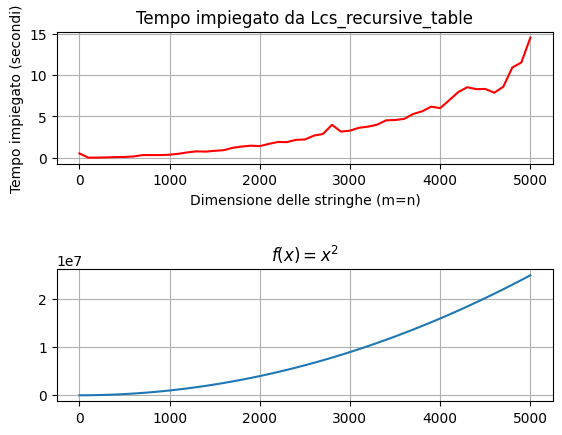
\includegraphics[width=0.5\textwidth]{LCS_recursive_table test.png}
    \caption{Test algoritmo ricorsivo tabella}
    \label{fig:lcs_recursive_table_test}
\end{figure}
\section{Conclusioni}
Abbiamo analizzato 4 possibili algoritmi per calcolare Lcs, l'algoritmo "brute-force", che per efficienza è il peggiore tra quelli esaminati (complessità $\Theta(n*2^m)$) , l'algoritmo ricorsivo, che migliora il precedente (complessità $\Theta(2^n)$),ma che nella sua versione con "memoization" riesce a raggiungere buone prestazioni (complessità $\Theta(n^2)$), e infine il migliore tra i menzionati, ovvero l'algoritmo iterativo (complessità $\Theta(n^2)$) che consente non solo di stabilire la lunghezza della LCS, ma anche i caratteri da cui è formata.


\end{document}
